%----------------------------------------------------------------------------------------
% LENGTE, OPPERVLAKTE EN VOLUME. Alle opgaven zijn eigen werk.
%
% Opbouw: Probleem, Start, leerstof, en op een nieuwe pagina de Opdrachten, Koppel en Test jezelf.
% Labels van dit hoofdstuk beginnen met h3-.
%----------------------------------------------------------------------------------------

\mychapter{3}{Lengte, oppervlakte en volume}

\begin{probleem}
\naast{In het profiel van een fietsband zit een steentje vast. Het wiel heeft een straal van 35~cm, en de fietser rijdt 1~km rechtdoor. Het steentje draait mee met het wiel en schuift tegelijk mee met de fiets: het beschrijft een rij bogen. Hoeveel meter legt het steentje af? Meer dan 1~km, want het maakt een omweg. Maar hoeveel meer? De formule voor de booglengte uit Integralen helpt niet, want de baan is gegeven met een parameter, en niet als grafiek van een functie.}{\begin{tikzpicture}[scale=.36,font=\scriptsize]
  \draw[lijngrijs] (-.3,0) -- (13,0);
  \pkromme{0}{12.5664}{\t-sin(\t r)}{1-cos(\t r)}
  \draw[lijngrijs] (8.5,1) circle (1);
  \fill (8.5,1) circle (2pt);
  \fill[fel!80!black] ({8.5-sin(8.5 r)},{1-cos(8.5 r)}) circle (4pt);
  \draw[->,lijngrijs] (9.8,1) -- (11.2,1);
  \draw[lijngrijs,|-|] (0,-.5) -- (6.2832,-.5) node[midway,below] {$2\pi R$};
\end{tikzpicture}}
\end{probleem}

\lkr{Leerplan Complementair (III-WiCo-d): LPD 19, met de drie wenken (de opbouw van de formules, de oppervlakte binnen een poolkromme met de lemniscaat, de cardioïde, het bifolium en het trifolium, en het volume van een omwentelingslichaam) en LPD 20 (de manteloppervlakte, met krommen in cartesische vergelijking zoals de wenk voorstelt; de vorm met een parameter staat in een opdracht van niveau 3). Voorkennis uit pakket 4: booglengte en omwentelingsvolume in cartesische vorm (Integralen, hoofdstuk 4), de mantel van een kegel (2de graad), en uit dit boek de primitieven van hoofdstuk 2. Parametervoorstellingen, de snelheidsvector, poolcoördinaten, de cycloïde, de cardioïde, de lemniscaat en rozen komen uit de module Krommen en meetkundige plaatsen. Wie die module niet volgde, krijgt hier telkens een korte herhaling; reken dan op een extra les. Het probleem is dat van Krommen, hoofdstuk 1, met een nieuwe vraag.}

In de cursus Integralen berekende je de lengte van een grafiek, de oppervlakte eronder en het volume als die grafiek om een as wentelt. Telkens was de kromme de grafiek van een functie $y = f(x)$. Maar veel krommen zijn geen grafiek: een cirkel, een cycloïde of een cardioïde gaan op en neer, of keren terug. Die beschrijf je beter met een parameter, of in poolcoördinaten. In dit hoofdstuk passen we de formules aan. Het idee blijft hetzelfde: snij in kleine stukjes, schrijf de bijdrage van een stukje, tel op. Op het einde komt er een nieuwe grootheid bij: de oppervlakte van de wand van een omwentelingslichaam.

\begin{oefeningen}[Start]
\oef{h3-start-1}

\oef{h3-verken}
\end{oefeningen}

\lkr{Oefening \ref{oef:h3-verken} bouwt de formule voor de booglengte met een parameter zelf op, met een gebroken lijn, zoals in Integralen. Laat leerlingen opmerken dat de som van de koorden een benadering is van de afgelegde weg, en dat die bij een snelheid van $5$ per tijdseenheid gewoon $5 \cdot$ tijd is.}

%========================================================================================
\section{Booglengte}

\subsection{Een kromme met een parameter}

Eerst een korte herhaling. Een \textit{parametervoorstelling} $x = x(t)$, $y = y(t)$ beschrijft een punt dat beweegt: op tijdstip $t$ is het in $\bigl(x(t), y(t)\bigr)$. Zijn snelheidsvector is $\bigl(x'(t), y'(t)\bigr)$, en de lengte daarvan, $\sqrt{x'(t)^2 + y'(t)^2}$, is de snelheid. Zo beschrijft een punt op de rand van een wiel met straal $R$ dat over een rechte rolt, de cycloïde $x = R(t - \sin t)$, $y = R(1 - \cos t)$, met $t$ de hoek waarover het wiel gedraaid is.

Hoe lang is de baan tussen $t = \alpha$ en $t = \beta$? Verdeel $[\alpha, \beta]$ in kleine stukjes $\Delta t$. Op zo'n stukje gaat $x$ ongeveer met $x'(t)\,\Delta t$ vooruit en $y$ met $y'(t)\,\Delta t$, en Pythagoras geeft de lengte van de koorde. Je kunt het ook zo zien: in een korte tijd is de afgelegde weg ongeveer de snelheid maal de tijd.

\figuren{\begin{tikzpicture}[scale=1.5,font=\scriptsize]
  \kromme{0}{3}{0.25*(\x)^2}
  \draw[accent,dashed] (1,.25) -- (2.3,1.3225);
  \draw[lijngrijs] (1,.25) -- (2.3,.25) -- (2.3,1.3225);
  \fill[accent] (1,.25) circle (1.3pt) (2.3,1.3225) circle (1.3pt);
  \node[above left] at (1,.25) {$t$};
  \node[above left] at (2.3,1.3225) {$t + \Delta t$};
  \node[below] at (1.65,.25) {$\Delta x \approx x'(t)\,\Delta t$};
  \node[right] at (2.3,.8) {$\Delta y \approx y'(t)\,\Delta t$};
\end{tikzpicture}}

\begin{theorie}
\begin{stelling}{Booglengte met een parameter}
Zijn $x'$ en $y'$ continu op $[\alpha, \beta]$, en doorloopt het punt de kromme één keer, dan is haar lengte

\vspace{1mm}
\qquad $\formule{L = \int_\alpha^\beta \sqrt{x'(t)^2 + y'(t)^2}\dt}$
\end{stelling}

\begin{bewijs}
Verdeel $[\alpha, \beta]$ in $n$ delen met breedte $\Delta t$, en vervang de kromme door de gebroken lijn door de punten met parameter $t_0, t_1, \ldots, t_n$. Volgens de stelling van Lagrange is $\Delta x = x'(c_k)\,\Delta t$ en $\Delta y = y'(d_k)\,\Delta t$ voor zekere $c_k$ en $d_k$ in het $k$-de deel, dus de $k$-de koorde heeft lengte
\bewijsregel{\sqrt{\Delta x^2 + \Delta y^2} = \sqrt{x'(c_k)^2 + y'(d_k)^2}\;\Delta t .}
Waren $c_k$ en $d_k$ gelijk, dan was de som van die lengtes een Riemannsom van $\sqrt{x'^2 + y'^2}$. Ze liggen wel in hetzelfde deel, en omdat $y'$ continu is, verschilt $y'(d_k)$ voor kleine $\Delta t$ willekeurig weinig van $y'(c_k)$. Dat het verschil van de sommen dan echt naar 0 gaat, vraagt een sterkere vorm van continuïteit die we hier aanvaarden. Voor $n \to +\infty$ volgt
\bewijsregel{L = \lim_{n \to +\infty} \sum_{k=1}^n \sqrt{x'(c_k)^2 + y'(c_k)^2}\;\Delta t = \ig_\alpha^\beta \sqrt{x'(t)^2 + y'(t)^2}\dt .}
\end{bewijs}
\end{theorie}

In woorden: de lengte van de baan is de integraal van de snelheid. Neem je $x = t$ en $y = f(t)$, dan staat er $\int \sqrt{1 + f'(t)^2}\dt$: de formule uit Integralen is een bijzonder geval. Eerst een controle met een kromme waarvan je de lengte al kent.

\voorbeeld{}{Bereken de omtrek van de cirkel $x = R\cos t$, $y = R\sin t$ met de formule.\label{vb:h3-cirkel}}{%
\uitleg{Voor $t \in [0, 2\pi]$ gaat het punt één keer rond. De snelheid blijkt constant.}
\begin{stappen}
x'(t)^2 + y'(t)^2 = R^2\sin^2 t + R^2\cos^2 t = R^2 & De afgeleiden zijn $-R\sin t$ en $R\cos t$. \\[1ex]
L = \ig_0^{2\pi} R\dt = 2\pi R & De bekende omtrek. Laat je $t$ tot $4\pi$ lopen, dan vind je $4\pi R$: het punt gaat twee keer rond.
\end{stappen}}

\voorbeeld{}{Bereken de lengte van één boog van de cycloïde $x = R(t - \sin t)$, $y = R(1 - \cos t)$.\label{vb:h3-cycloide}}{%
\uitleg{Eén boog hoort bij één omwenteling: $t \in [0, 2\pi]$. Onder de wortel verschijnt $1 - \cos t$, en een formule van Carnot maakt daar een kwadraat van.}
\naast{\begin{stappenvrij}{7.4cm}{3.6cm}
x'^2 + y'^2 = R^2(1 - \cos t)^2 + R^2\sin^2 t & $x' = R(1 - \cos t)$, $y' = R\sin t$. \\[1ex]
= R^2(2 - 2\cos t) = 4R^2\sin^2\dfrac t2 & Uitwerken; Carnot: $1 - \cos t = 2\sin^2\tfrac t2$. \\[2.5ex]
L = \ig_0^{2\pi} 2R\sin\dfrac t2\dt = \grens{-4R\cos\dfrac t2}{0}{2\pi} = 8R & Op $[0, 2\pi]$ is $\sin\tfrac t2 \geqslant 0$.
\end{stappenvrij}}{\begin{tikzpicture}[scale=.36,font=\scriptsize]
  \draw[lijngrijs] (-.3,0) -- (6.8,0);
  \pkromme[very thick]{0}{6.2832}{\t-sin(\t r)}{1-cos(\t r)}
  \draw[lijngrijs,|-|] (0,-.6) -- (6.2832,-.6) node[midway,below] {$2\pi R$};
\end{tikzpicture}}
De lengte is precies $8R$, een geheel veelvoud van de straal. Christopher Wren vond dat resultaat in 1658, nog vóór de integraalrekening bestond.}

\begin{werkwijze}
Zoek het interval van de parameter waarop de kromme één keer doorlopen wordt. Bereken $x'(t)^2 + y'(t)^2$ en vereenvoudig: zoek een kwadraat onder de wortel, met $\sin^2 + \cos^2 = 1$ of een formule van Carnot. Let op het teken als je de wortel trekt. Lukt exact rekenen niet, gebruik dan het rekentoestel.
\end{werkwijze}

\nujij{Bereken de lengte van $x = t^2$, $y = t^3$ voor $t \in [0, 1]$.}{$\sqrt{4t^2 + 9t^4} = t\sqrt{4 + 9t^2}$: \ $\tfrac{1}{27}\bigl(13\sqrt{13} - 8\bigr) \approx 1{,}440$.}

\begin{oefeningen}
\oef{h3-boog}
\end{oefeningen}

\subsection{Terug naar het probleem}

\voorbeeld{}{Terug naar het probleem. In het profiel van een fietsband zit een steentje vast. Het wiel heeft een straal van 35~cm, en de fietser rijdt 1~km rechtdoor. Het steentje draait mee met het wiel en schuift tegelijk mee met de fiets: het beschrijft een rij bogen. Hoeveel meter legt het steentje af?\label{vb:h3-terug}}{%
\uitleg{Per omwenteling rijdt de fiets de omtrek $2\pi R$ vooruit, en legt het steentje één boog van de cycloïde af: $8R$. Het quotiënt hangt dus niet van $R$ af.}
\begin{stappen}
\dfrac{8R}{2\pi R} = \dfrac{4}{\pi} \approx 1{,}273 & Weg van het steentje gedeeld door weg van de fiets. \\[2ex]
1000 \cdot \dfrac{4}{\pi} \approx 1273 \text{ m} & Bij elke straal van het wiel.
\end{stappen}
Het steentje legt ongeveer 1273~m af, 27\,\% meer dan de fiets. Toch staat het even stil telkens als het de grond raakt: daar is zijn snelheid 0. Bovenaan gaat het twee keer zo snel als de fiets. Gemiddeld gaat het $\tfrac{4}{\pi}$ keer zo snel.}

\begin{oefeningen}
\oef{h3-fiets}
\end{oefeningen}

\subsection{Een kromme in poolcoördinaten}

Ook dit eerst kort herhaald. Een punt met \textit{poolcoördinaten} $[r, \theta]$ ligt op afstand $r$ van de pool $O$, in de richting met hoek $\theta$, en heeft cartesische coördinaten $x = r\cos\theta$, $y = r\sin\theta$. Een \textit{poolvergelijking} $r = f(\theta)$ geeft bij elke richting een afstand. Zo is $r = 2a(1 - \cos\theta)$ de cardioïde, de baan van een punt op een munt die rond een even grote munt rolt. Hoe lang is die kromme? Schrijf ze met $\theta$ als parameter: $x = f(\theta)\cos\theta$ en $y = f(\theta)\sin\theta$. Dan geldt de vorige formule, en die wordt verrassend eenvoudig.

\begin{theorie}
\begin{stelling}{Booglengte in poolcoördinaten}
Is $f'$ continu op $[\alpha, \beta]$, en wordt de kromme $r = f(\theta)$ één keer doorlopen, dan is haar lengte

\vspace{1mm}
\qquad $\formule{L = \int_\alpha^\beta \sqrt{r^2 + r'^2}\dth}$ \qquad met $r = f(\theta)$ en $r' = f'(\theta)$.
\end{stelling}

\begin{bewijs}
Met $\theta$ als parameter is $x = r\cos\theta$ en $y = r\sin\theta$, dus volgens de productregel
\bewijsregel{x' = r'\cos\theta - r\sin\theta, \qquad y' = r'\sin\theta + r\cos\theta .}
Kwadrateer en tel op. De dubbele producten $\mp 2rr'\sin\theta\cos\theta$ vallen weg, en met $\sin^2\theta + \cos^2\theta = 1$ blijft
\bewijsregel{x'^2 + y'^2 = r'^2 + r^2 .}
\end{bewijs}
\end{theorie}

\naast{De formule is ook te zien. Draait de hoek een klein beetje, $\Delta\theta$, dan schuift het punt in de richting loodrecht op de voerstraal ongeveer $r\,\Delta\theta$ op, zoals op een cirkelboog. In de richting van de voerstraal verandert de afstand met ongeveer $r'\,\Delta\theta$. Die twee verplaatsingen staan loodrecht op elkaar: Pythagoras.}{\begin{tikzpicture}[scale=1.1,font=\scriptsize]
  \fill (0,0) circle (1.2pt) node[below left] {$O$};
  \draw[lijngrijs] (0,0) -- (20:2.3) (0,0) -- (45:2.9);
  \draw[accent,thick] plot[domain=12:52,samples=40,smooth,variable=\t] (\t:{2+0.02*(\t-20)});
  \draw[grijs,dashed] (20:2) arc[start angle=20,end angle=45,radius=2];
  \draw[fel!80!black,very thick] (45:2) -- (45:2.5);
  \fill[accent] (20:2) circle (1.3pt) (45:2.5) circle (1.3pt);
  \node[below right] at (33:2) {$r\,\Delta\theta$};
  \node[left] at (45:2.3) {$r'\,\Delta\theta$};
  \draw (.5,0) arc[start angle=0,end angle=20,radius=.5];
  \node at (.72,.12) {$\theta$};
  \draw (20:1) arc[start angle=20,end angle=45,radius=1];
  \node at (33:1.2) {$\Delta\theta$};
\end{tikzpicture}}

\voorbeeld{}{Bereken de lengte van de cardioïde $r = 2a(1 - \cos\theta)$.\label{vb:h3-cardioide}}{%
\uitleg{Voor $\theta \in [0, 2\pi]$ wordt de kromme één keer doorlopen. Onder de wortel komt weer $1 - \cos\theta$, net zoals bij de cycloïde.}
\naast{\begin{stappenvrij}{7.6cm}{3.4cm}
r^2 + r'^2 = 4a^2\bigl((1 - \cos\theta)^2 + \sin^2\theta\bigr) & $r' = 2a\sin\theta$. \\[1ex]
= 8a^2(1 - \cos\theta) = 16a^2\sin^2\dfrac\theta2 & Zoals bij de cycloïde. \\[2.5ex]
L = \ig_0^{2\pi} 4a\sin\dfrac\theta2\dth = \grens{-8a\cos\dfrac\theta2}{0}{2\pi} = 16a & $\sin\tfrac\theta2 \geqslant 0$ op $[0, 2\pi]$.
\end{stappenvrij}}{\begin{tikzpicture}[scale=.42,font=\scriptsize]
  \draw[lijngrijs,thick,fill=black!6] (-1,0) circle (1);
  \poolkromme[very thick]{0}{360}{2*(1-cos(\t))}
  \fill (0,0) circle (2.5pt) node[right] {$O$};
\end{tikzpicture}}
De cardioïde van twee munten met straal $a$ is $16a$ lang, acht keer de diameter van een munt.}

Niet elke kromme geeft zo'n mooi kwadraat. Bij de spiraal van Archimedes heb je de primitieven van hoofdstuk 2 nodig.

\voorbeeld{}{Bereken de lengte van de eerste winding van de spiraal $r = \theta$, voor $\theta \in [0, 2\pi]$.\label{vb:h3-spiraal}}{%
\uitleg{Hier is $r' = 1$, dus staat er $\sqrt{\theta^2 + 1}$: de vorm $\sqrt{x^2 + a^2}$ uit hoofdstuk 2, met $a = 1$.}
\naast{\begin{stappenvrij}{7.2cm}{3cm}
L = \ig_0^{2\pi} \sqrt{\theta^2 + 1}\dth & $r^2 + r'^2 = \theta^2 + 1$. \\[2.5ex]
= \dfrac12\Bigl[\theta\sqrt{\theta^2 + 1} + \ln\bigl(\theta + \sqrt{\theta^2 + 1}\bigr)\Bigr]_0^{2\pi} & De primitieve van $\sqrt{x^2 + a^2}$. \\[3ex]
= \pi\sqrt{4\pi^2 + 1} + \dfrac12\ln\bigl(2\pi + \sqrt{4\pi^2 + 1}\bigr) \approx 21{,}26 & In 0 is de primitieve 0.
\end{stappenvrij}}{\begin{tikzpicture}[scale=.24,font=\scriptsize]
  \poolrooster{6.4}{2}
  \poolkromme[very thick]{0}{360}{\t*pi/180}
\end{tikzpicture}}
Controle: de spiraal ligt tussen de pool en de cirkel met straal $2\pi$, met omtrek $4\pi^2 \approx 39{,}5$. Haar lengte is iets meer dan de helft daarvan.}

\begin{werkwijze}
Bereken $r'$, en dan $r^2 + r'^2$. Vereenvoudig tot een kwadraat als dat kan, of herken een vorm uit hoofdstuk 2. Kies het interval van $\theta$ waarop de kromme één keer doorlopen wordt.
\end{werkwijze}

\nujij{De kromme $r = 2\cos\theta$, met $\theta \in [0, \pi]$, is een cirkel. Bereken haar lengte met de formule.}{$r^2 + r'^2 = 4\cos^2\theta + 4\sin^2\theta = 4$: \ $L = 2\pi$. Een cirkel met diameter 2.}

\begin{oefeningen}
\oef{h3-boogpool}
\end{oefeningen}

%========================================================================================
\section{Oppervlakte}

\subsection{Met een parameter}

Hoe groot is de oppervlakte onder één boog van de cycloïde? Bij een grafiek is dat $\int y\dx$. Hier hangen $x$ en $y$ allebei van $t$ af. Lees dat als een substitutie $x = x(t)$, zoals in hoofdstuk 2: dan wordt $\mathrm{d}x = x'(t)\dt$.

\begin{theorie}
\begin{stelling}{Oppervlakte met een parameter}
Is $x(t)$ stijgend met een continue afgeleide op $[\alpha, \beta]$, en $y(t) \geqslant 0$, dan is de oppervlakte tussen de kromme, de $x$-as en de verticale rechten door de eindpunten

\vspace{1mm}
\qquad $\formule{A = \int_\alpha^\beta y(t)\,x'(t)\dt}$
\end{stelling}

\begin{bewijs}
Noem $a = x(\alpha)$ en $b = x(\beta)$. Omdat $x(t)$ stijgt, is de kromme de grafiek van een functie $f$ met $f(x(t)) = y(t)$, en is $A = \int_a^b f(x)\dx$. De substitutie $x = x(t)$ uit hoofdstuk 2 geeft
\bewijsregel{\ig_a^b f(x)\dx = \ig_\alpha^\beta f\bigl(x(t)\bigr)\,x'(t)\dt = \ig_\alpha^\beta y(t)\,x'(t)\dt .}
\end{bewijs}
\end{theorie}

Daalt $x(t)$, dan doorloop je de kromme van rechts naar links, en krijg je de oppervlakte met een minteken. Neem dan de absolute waarde, of keer de grenzen om.

\voorbeeld{}{Bereken de oppervlakte onder één boog van de cycloïde $x = R(t - \sin t)$, $y = R(1 - \cos t)$.\label{vb:h3-oppcycloide}}{%
\uitleg{Op $[0, 2\pi]$ stijgt $x(t)$, want $x'(t) = R(1 - \cos t) \geqslant 0$. Dus de formule geldt meteen.}
\naast{\begin{stappenvrij}{7.6cm}{3.4cm}
A = \ig_0^{2\pi} R(1 - \cos t) \cdot R(1 - \cos t)\dt & $y(t) \cdot x'(t)$. \\[2.5ex]
= R^2 \ig_0^{2\pi} \Bigl(1 - 2\cos t + \dfrac{1 + \cos 2t}{2}\Bigr)\dt & Uitwerken, en Carnot. \\[2.5ex]
= R^2 \Bigl(2\pi - 0 + \pi\Bigr) = 3\pi R^2 & Over een volle periode geven de cosinussen 0.
\end{stappenvrij}}{\begin{tikzpicture}[scale=.36,font=\scriptsize]
  \fill[accent!30] plot[domain=0:6.2832,samples=80,variable=\t] ({\t-sin(\t r)},{1-cos(\t r)}) -- cycle;
  \draw[lijngrijs] (-.3,0) -- (6.8,0);
  \pkromme{0}{6.2832}{\t-sin(\t r)}{1-cos(\t r)}
  \draw[lijngrijs] (3.1416,1) circle (1);
\end{tikzpicture}}
Drie keer de oppervlakte van het wiel. Galilei probeerde het in 1599 te vinden door stukken uitgesneden metaal te wegen.}

Bij een gesloten kromme loopt $x(t)$ heen en terug. Splits ze dan in stukken waarop $x$ stijgt of daalt, of gebruik een symmetrie.

\voorbeeld{}{De kromme $x = t^2$, $y = t^3 - 4t$ heeft een lus voor $t \in [-2, 2]$. Bereken de oppervlakte binnen de lus.\label{vb:h3-lus}}{%
\uitleg{Bij $t$ en $-t$ hoort dezelfde $x$ en een tegengestelde $y$: de lus is symmetrisch ten opzichte van de $x$-as. Voor $t \in [-2, 0]$ is $y = t(t^2 - 4) \geqslant 0$: dat is de bovenste helft. Daar daalt $x$ van 4 naar 0.}
\naast{\begin{stappenvrij}{7.6cm}{3.4cm}
A_{\text{boven}} = -\ig_{-2}^0 (t^3 - 4t) \cdot 2t\dt & $x$ daalt: een minteken. \\[2.5ex]
= -2\grens{\dfrac{t^5}{5} - \dfrac{4t^3}{3}}{-2}{0} = \dfrac{128}{15} & $-2\bigl(0 - (-\tfrac{32}{5} + \tfrac{32}{3})\bigr)$. \\[3ex]
A = 2 \cdot \dfrac{128}{15} = \dfrac{256}{15} \approx 17{,}1 & De twee helften.
\end{stappenvrij}}{\begin{tikzpicture}[scale=.36,font=\scriptsize]
  \fill[accent!30] plot[domain=-2:2,samples=80,variable=\t] ({(\t)^2},{(\t)^3-4*\t}) -- cycle;
  \rooster{0}{1}{4}{-3}{1}{3}
  \pkromme{-2.25}{2.25}{(\t)^2}{(\t)^3-4*\t}
\end{tikzpicture}}}

\begin{werkwijze}
Ga na waar $x(t)$ stijgt en waar $y(t) \geqslant 0$. Bereken $\int y(t)\,x'(t)\dt$ op een interval waar $x$ stijgt; daalt $x$, zet er dan een minteken voor. Gebruik symmetrie om het rekenwerk te beperken.
\end{werkwijze}

\nujij{Bereken de oppervlakte van de ellips $x = 3\cos t$, $y = 2\sin t$ met de formule.}{Bovenste helft: $t$ van $\pi$ naar 0, waar $x$ stijgt: $\int_\pi^0 2\sin t \cdot (-3\sin t)\dt = 3\pi$. Samen $6\pi = \pi \cdot 3 \cdot 2$.}

\begin{oefeningen}
\oef{h3-opppar}
\end{oefeningen}

\subsection{In poolcoördinaten}

Bij een poolkromme snij je niet in verticale stroken, maar in smalle sectoren rond de pool. Waarom? Een kromme als de lemniscaat of een roos draait rond de pool, en een strook loodrecht op de $x$-as zou haar op een onhandige manier doorsnijden. Een cirkelsector met straal $r$ en middelpuntshoek $\Delta\theta$ heeft oppervlakte $\tfrac12 r^2\Delta\theta$: dat is de bouwsteen.

\begin{theorie}
\begin{stelling}{Oppervlakte in poolcoördinaten}
Is $f$ continu en $f(\theta) \geqslant 0$ op $[\alpha, \beta]$, met $\beta - \alpha \leqslant 2\pi$, dan is de oppervlakte van het gebied tussen de pool en de kromme $r = f(\theta)$ voor $\theta \in [\alpha, \beta]$

\vspace{1mm}
\qquad $\formule{A = \dfrac12\int_\alpha^\beta r^2\dth}$
\end{stelling}

\begin{bewijs}
Verdeel $[\alpha, \beta]$ in $n$ delen met breedte $\Delta\theta$. Op het $k$-de deel heeft $f$ een kleinste waarde $m_k$ en een grootste waarde $M_k$. Het stuk van het gebied tussen die twee richtingen bevat de sector met straal $m_k$ en ligt in de sector met straal $M_k$, dus
\bewijsregel{\tfrac12 m_k^2\,\Delta\theta \leqslant A_k \leqslant \tfrac12 M_k^2\,\Delta\theta .}
Tel op over $k$. Links staat een ondersom en rechts een bovensom van $\tfrac12 f^2$, en die gaan allebei naar $\tfrac12\int_\alpha^\beta f(\theta)^2\dth$. De oppervlakte $A = \sum A_k$ ligt ertussen, en is dus die integraal.
\end{bewijs}
\end{theorie}

\figuren{\begin{tikzpicture}[scale=1.4,font=\scriptsize]
  \fill (0,0) circle (1.2pt) node[below left] {$O$};
  \fill[accent!35] (0,0) -- (30:1.25) arc[start angle=30,end angle=45,radius=1.25] -- cycle;
  \draw[accent] (0,0) -- (30:1.25) arc[start angle=30,end angle=45,radius=1.25] -- cycle;
  \draw[grijs,dashed] (0,0) -- (45:1.62) arc[start angle=45,end angle=30,radius=1.62] -- cycle;
  \draw[accent,thick] plot[domain=0:80,samples=60,smooth,variable=\t] (\t:{1+0.012*\t});
  \node at (37:.7) {$m_k$};
  \node[right] at (37:1.65) {$M_k$};
  \draw[->,grijs] (0,0) -- (2.1,0);
\end{tikzpicture}}

\voorbeeld{}{Bereken de oppervlakte binnen de lemniscaat van Bernoulli $r^2 = 2c^2\cos 2\theta$.\label{vb:h3-lemniscaat}}{%
\uitleg{Een punt bestaat alleen waar $\cos 2\theta \geqslant 0$. De rechterlus hoort bij $\theta \in \bigl[-\tfrac{\pi}{4}, \tfrac{\pi}{4}\bigr]$, de linkerlus is haar spiegelbeeld. Hier staat $r^2$ al in de vergelijking: dat is handig.}
\naast{\begin{stappenvrij}{7.2cm}{3.4cm}
A_{\text{lus}} = \dfrac12\ig_{-\pi/4}^{\pi/4} 2c^2\cos 2\theta\dth & Eén lus. \\[2.5ex]
= c^2\grens{\dfrac{\sin 2\theta}{2}}{-\pi/4}{\pi/4} = c^2 & $\tfrac12 - \bigl(-\tfrac12\bigr) = 1$. \\[2.5ex]
A = 2c^2 & Twee lussen.
\end{stappenvrij}}{\begin{tikzpicture}[scale=.95,font=\scriptsize]
  \fill[accent!30] plot[domain=-45:45,samples=60,variable=\t] (\t:{sqrt(2*cos(2*\t))}) -- cycle;
  \fill[accent!30] plot[domain=135:225,samples=60,variable=\t] (\t:{sqrt(2*cos(2*\t))}) -- cycle;
  \draw[->,grijs] (-1.7,0) -- (1.8,0);
  \draw[accent,thick] plot[domain=-45:45,samples=60,smooth,variable=\t] (\t:{sqrt(2*cos(2*\t))});
  \draw[accent,thick] plot[domain=135:225,samples=60,smooth,variable=\t] (\t:{sqrt(2*cos(2*\t))});
  \fill (-1,0) circle (1.2pt) (1,0) circle (1.2pt);
  \node[below] at (1,0) {$F_2$};
  \node[below] at (-1,0) {$F_1$};
\end{tikzpicture}}
Een verrassend eenvoudige uitkomst: de oppervlakte van het vierkant met diagonaal $[F_1F_2]$, want die diagonaal is $2c$ lang.}

\voorbeeld{}{Bereken de oppervlakte binnen het trifolium $r = a\cos 3\theta$.\label{vb:h3-trifolium}}{%
\uitleg{Een blad begint en eindigt in de pool, waar $r = 0$: dat is bij $3\theta = \pm\tfrac{\pi}{2}$. Eén blad hoort dus bij $\theta \in \bigl[-\tfrac{\pi}{6}, \tfrac{\pi}{6}\bigr]$, en er zijn drie gelijke bladen.}
\naast{\begin{stappenvrij}{7.2cm}{3.4cm}
A_{\text{blad}} = \dfrac12\ig_{-\pi/6}^{\pi/6} a^2\cos^2 3\theta\dth & Eén blad, waar $r \geqslant 0$. \\[2.5ex]
= \dfrac{a^2}{2}\grens{\dfrac\theta2 + \dfrac{\sin 6\theta}{12}}{-\pi/6}{\pi/6} = \dfrac{\pi a^2}{12} & Carnot met $6\theta$; de sinus geeft 0. \\[2.5ex]
A = 3 \cdot \dfrac{\pi a^2}{12} = \dfrac{\pi a^2}{4} & Drie bladen.
\end{stappenvrij}}{\begin{tikzpicture}[scale=1.05,font=\scriptsize]
  \draw[lijngrijs,dashed] (0,0) circle (1);
  \fill[accent!30] plot[domain=0:180,samples=120,variable=\t] (\t:{cos(3*\t)}) -- cycle;
  \poolkromme{0}{180}{cos(3*\t)}
  \fill (0,0) circle (1pt);
\end{tikzpicture}}
Het klaverblad beslaat precies een kwart van de cirkel $r = a$ waarin het past.}

\begin{werkwijze}
Zoek waar $r = 0$: daar begint en eindigt een lus of een blad. Kies een interval van $\theta$ waarop het gebied één keer doorlopen wordt, met $r \geqslant 0$. Bereken $\tfrac12 \int r^2\dth$, en gebruik symmetrie.
\end{werkwijze}

\nujij{Bereken de oppervlakte binnen de cirkel $r = 2\cos\theta$, met $\theta \in \bigl[-\tfrac{\pi}{2}, \tfrac{\pi}{2}\bigr]$.}{$\tfrac12 \int 4\cos^2\theta\dth = 2 \cdot \tfrac{\pi}{2} = \pi$: een cirkel met straal 1.}

\begin{oefeningen}
\oef{h3-opppool}
\end{oefeningen}

%========================================================================================
\section{Volume en manteloppervlakte}

\subsection{Volume met een parameter}

Wentel een kromme met een parameter om de $x$-as. Het volume uit Integralen is $\pi\int y^2\dx$, en de substitutie $x = x(t)$ geeft meteen de vorm met een parameter, net als bij de oppervlakte.

\begin{theorie}
\begin{stelling}{Volume met een parameter}
Is $x(t)$ stijgend met een continue afgeleide op $[\alpha, \beta]$, dan is het volume van het lichaam dat ontstaat als de kromme om de $x$-as wentelt

\vspace{1mm}
\qquad $\formule{V = \pi\int_\alpha^\beta y(t)^2\,x'(t)\dt}$
\end{stelling}

\begin{bewijs}
Zoals bij de oppervlakte is de kromme de grafiek van een functie $f$ met $f(x(t)) = y(t)$, en de substitutie $x = x(t)$ geeft
\bewijsregel{V = \pi\ig_a^b f(x)^2\dx = \pi\ig_\alpha^\beta y(t)^2\,x'(t)\dt .}
\end{bewijs}
\end{theorie}

\voorbeeld{}{Eén boog van de cycloïde $x = R(t - \sin t)$, $y = R(1 - \cos t)$ wentelt om de $x$-as. Bereken het volume.\label{vb:h3-volume}}{%
\uitleg{Op $[0, 2\pi]$ stijgt $x(t)$. Nu staat er $(1 - \cos t)^3$: werk uit, en ken de integralen van de machten van $\cos t$ over een volle periode.}
\naast{\begin{stappenvrij}{7.6cm}{3.2cm}
V = \pi\ig_0^{2\pi} R^2(1 - \cos t)^2 \cdot R(1 - \cos t)\dt & $y^2 \cdot x'$. \\[2.5ex]
= \pi R^3\ig_0^{2\pi} (1 - 3\cos t + 3\cos^2 t - \cos^3 t)\dt & Het binomium van Newton. \\[2.5ex]
= \pi R^3(2\pi - 0 + 3\pi - 0) = 5\pi^2R^3 & $\int_0^{2\pi} \cos^2 t\dt = \pi$; $\cos t$ en $\cos^3 t$ geven 0.
\end{stappenvrij}}{\begin{tikzpicture}[scale=.36,font=\scriptsize]
  \fill[accent!30] plot[domain=0:6.2832,samples=80,variable=\t] ({\t-sin(\t r)},{1-cos(\t r)}) -- plot[domain=6.2832:0,samples=80,variable=\t] ({\t-sin(\t r)},{-(1-cos(\t r))}) -- cycle;
  \pkromme{0}{6.2832}{\t-sin(\t r)}{1-cos(\t r)}
  \pkromme{0}{6.2832}{\t-sin(\t r)}{-(1-cos(\t r))}
  \draw[accent,fill=accent!45] (3.1416,0) ellipse (.3 and 2);
  \draw[->,lijngrijs] (-.5,0) -- (7,0);
\end{tikzpicture}}
Dat $\int_0^{2\pi} \cos^3 t\dt = 0$, volgt uit de symmetrie: $\cos^3(\pi - t) = -\cos^3 t$.}

\begin{werkwijze}
Controleer dat $x(t)$ stijgt, of keer anders de grenzen om. Schrijf $\pi\int y(t)^2\,x'(t)\dt$ en werk uit.
\end{werkwijze}

\nujij{De halve cirkel $x = r\cos t$, $y = r\sin t$ met $t \in [0, \pi]$ wentelt om de $x$-as. Toon aan dat het volume $\tfrac43\pi r^3$ is.}{$x$ stijgt als $t$ van $\pi$ naar 0 gaat: $\pi\int_\pi^0 r^2\sin^2 t \cdot (-r\sin t)\dt = \pi r^3 \int_0^\pi \sin^3 t\dt = \tfrac43\pi r^3$, met $\sin^3 t = \sin t\,(1 - \cos^2 t)$.}

\begin{oefeningen}
\oef{h3-volume}
\end{oefeningen}

\subsection{Manteloppervlakte}

Hoeveel verf heb je nodig voor de buitenkant van een vaas? Daarvoor heb je de oppervlakte van de wand nodig, de \textit{manteloppervlakte}. Voor een cilinder en een kegel ken je ze: $2\pi rh$ en $\pi rs$, met $s$ de schuine zijde. Rol je een kegelmantel af, dan krijg je een cirkelsector met straal $s$ en booglengte $2\pi r$, en die heeft oppervlakte $\tfrac12 \cdot s \cdot 2\pi r$. Een afgeknotte kegel is een grote kegel min een kleine. Met stralen $r_1$ en $r_2$ en schuine zijde $s$ heeft hij manteloppervlakte $\pi(r_1 + r_2)\,s$: de omtrek van de middelste cirkel maal $s$. Reken dat na in opdracht \ref{oef:h3-o14}.

\naast{Snij een omwentelingslichaam nu in smalle schijven loodrecht op de as. De wand van zo'n schijf is bijna een afgeknotte kegel, met stralen $f(x_{k-1})$ en $f(x_k)$. Zijn schuine zijde is niet $\Delta x$, maar de koorde van de grafiek: $\sqrt{1 + f'(c_k)^2}\,\Delta x$, zoals bij de booglengte. Dat verschil is belangrijk: rekenen met $\Delta x$ zou een cilinder geven in plaats van een schuine wand.}{\begin{tikzpicture}[x=1.25cm,y=.8cm,font=\scriptsize]
  \fill[fel!45] (1.4,1.29) -- (2.1,1.535) -- (2.1,-1.535) -- (1.4,-1.29) -- cycle;
  \draw[->,lijngrijs] (-.1,0) -- (3.3,0) node[right,text=black] {$x$};
  \kromme{.2}{3}{0.8+0.35*\x}
  \draw[accent,dashed] (.2,-.87) -- (3,-1.85);
  \draw[accent] (.2,0) ellipse (.12 and .87) (3,0) ellipse (.2 and 1.85);
  \draw[accent] (1.4,0) ellipse (.15 and 1.29) (2.1,0) ellipse (.17 and 1.535);
  \draw[fel!80!black,very thick] (1.4,1.29) -- (2.1,1.535);
  \node[above] at (1.75,1.45) {$s$};
  \draw[lijngrijs,|-|] (1.4,-2.1) -- (2.1,-2.1) node[midway,below] {$\Delta x$};
\end{tikzpicture}}

\begin{theorie}
\begin{stelling}{Manteloppervlakte}
Is $f(x) \geqslant 0$ met $f'$ continu op $[a, b]$, dan heeft het lichaam dat ontstaat als de grafiek van $f$ om de $x$-as wentelt, als manteloppervlakte

\vspace{1mm}
\qquad $\formule{S = 2\pi\int_a^b f(x)\sqrt{1 + f'(x)^2}\dx}$
\end{stelling}

\begin{bewijs}
Verdeel $[a, b]$ in $n$ delen met breedte $\Delta x$. Vervang de grafiek door de gebroken lijn door de punten $\bigl(x_k, f(x_k)\bigr)$. Wentelen geeft afgeknotte kegels, en de $k$-de heeft manteloppervlakte
\bewijsregel{\pi\bigl(f(x_{k-1}) + f(x_k)\bigr)\sqrt{1 + f'(c_k)^2}\;\Delta x ,}
met $c_k$ uit de stelling van Lagrange, zoals bij de booglengte. Omdat $f$ continu is, liggen $f(x_{k-1})$ en $f(x_k)$ voor kleine $\Delta x$ allebei willekeurig dicht bij $f(c_k)$, en is het eerste deel ongeveer $2\pi f(c_k)$. Net als bij de booglengte aanvaarden we dat de som dan dezelfde limiet heeft als de Riemannsom $\sum 2\pi f(c_k)\sqrt{1 + f'(c_k)^2}\,\Delta x$, en dat is de integraal.
\end{bewijs}
\end{theorie}

In woorden: elk stukje boog $\Delta s$ beschrijft bij het wentelen een smalle band met omtrek $2\pi f(x)$, en dus oppervlakte $2\pi f(x)\,\Delta s$. Een eerste controle met een kegel.

\voorbeeld{}{De rechte $y = x$ op $[0, 1]$ wentelt om de $x$-as. Bereken de manteloppervlakte met de formule, en vergelijk met de formule $\pi rs$ voor een kegel.\label{vb:h3-kegel}}{%
\uitleg{Het lichaam is een kegel met straal 1 en schuine zijde $\sqrt2$. Dat laat ons ook de klassieke fout zien.}
\begin{stappen}
S = 2\pi\ig_0^1 x\sqrt{1 + 1}\dx = 2\pi\sqrt2 \cdot \dfrac12 = \pi\sqrt2 & $f'(x) = 1$. \\[2.5ex]
\pi rs = \pi \cdot 1 \cdot \sqrt2 & Dezelfde uitkomst. \\[1ex]
2\pi\ig_0^1 x\dx = \pi & Fout: zonder de wortel reken je met $\Delta x$ in plaats van $\Delta s$, en dat is te weinig.
\end{stappen}}

\voorbeeld{}{Toon aan dat een bol met straal $r$ oppervlakte $4\pi r^2$ heeft.\label{vb:h3-bol}}{%
\uitleg{Wentel de halve cirkel $f(x) = \sqrt{r^2 - x^2}$ op $[-r, r]$. Vereenvoudig eerst $f\sqrt{1 + f'^2} = \sqrt{f^2 + (ff')^2}$, dat is korter.}
\naast{\begin{stappenvrij}{7.4cm}{3.4cm}
f(x)f'(x) = -x & $f' = \tfrac{-x}{\sqrt{r^2 - x^2}}$. \\[1ex]
f\sqrt{1 + f'^2} = \sqrt{f^2 + (ff')^2} = \sqrt{r^2 - x^2 + x^2} = r & Een constante! \\[1ex]
S = 2\pi\ig_{-r}^r r\dx = 4\pi r^2 & Vier keer een grote cirkel.
\end{stappenvrij}}{\begin{tikzpicture}[scale=.55,font=\scriptsize]
  \draw[accent,thick] (0,0) circle (2);
  \draw[accent] (0,0) ellipse (2 and .45);
  \fill[fel!50] (.6,-1.908) -- (.6,1.908) -- (1.1,1.67) -- (1.1,-1.67) -- cycle;
  \draw[accent] (.6,0) ellipse (.2 and 1.908) (1.1,0) ellipse (.17 and 1.67);
  \draw[->,lijngrijs] (-2.5,0) -- (2.7,0);
\end{tikzpicture}}
Archimedes vond dit al: de bol heeft dezelfde oppervlakte als de mantel van de cilinder eromheen, met straal $r$ en hoogte $2r$. Omdat de integrand constant is, geldt meer: een schijf van de bol tussen twee evenwijdige vlakken op afstand $h$ heeft altijd mantel $2\pi rh$, waar je ook snijdt.}

\begin{werkwijze}
Bereken $f'(x)$ en $1 + f'(x)^2$, of meteen $f^2 + (ff')^2$. Vereenvoudig zoveel mogelijk. Bereken $2\pi\int_a^b f(x)\sqrt{1 + f'(x)^2}\dx$, exact of met het rekentoestel. Vergeet de wortel niet.
\end{werkwijze}

\nujij{De grafiek van $f(x) = \sqrt{x}$ op $[0, 2]$ wentelt om de $x$-as. Bereken de manteloppervlakte.}{$f^2 + (ff')^2 = x + \tfrac14$: \ $2\pi\int_0^2 \sqrt{x + \tfrac14}\dx = \tfrac{4\pi}{3}\bigl(\tfrac{27}{8} - \tfrac18\bigr) = \tfrac{13\pi}{3}$.}

\begin{oefeningen}
\oef{h3-mantel}
\end{oefeningen}

%========================================================================================
\opdrachtenkop

\begin{oefeningen}
\needspace{14\baselineskip}
\oef{h3-o1}

\oef{h3-o2}

\oef{h3-o3}

\oef{h3-o4}

\oef{h3-o5}

\oef{h3-o6}

\oef{h3-o7}

\oef{h3-o8}

\oef{h3-o9}

\oef{h3-o10}

\oef{h3-o11}

\oef{h3-o12}

\oef{h3-o13}

\oef{h3-o14}

\oef{h3-o15}

\oef{h3-o16}

\oef{h3-o17}

\oef{h3-o18}

\oef{h3-o19}

\oef{h3-o20}

\oef{h3-o21}
\end{oefeningen}

%----------------------------------------------------------------------------------------
% KOPPEL: verbanden met andere leerstof
%----------------------------------------------------------------------------------------
\needspace{20\baselineskip}
\opdrachtsectie{Koppel}

\lkr{Kegelsneden, Oppervlakken en Numerieke methodes zijn modules van het leerplan Complementair (Kegelsneden ook van GO! en de keuze van de school): kijk na of ze al gezien zijn. De oefeningen geven de nodige vergelijkingen en de regel van Simpson zelf.}

\begin{oefeningen}
\oef{h3-koppel-1}

\oef{h3-koppel-2}

\oef{h3-koppel-3}
\end{oefeningen}

%----------------------------------------------------------------------------------------
\needspace{30\baselineskip} % de test en het schema Fout? Herhaal samen op een pagina
\opdrachtsectie{Test jezelf}

\begin{oefeningen}
\oef{h3-t1}

\oef{h3-t2}

\oef{h3-t3}

\oef{h3-t4}

\oef{h3-t5}

\oef{h3-t6}

\oef{h3-t7}
\end{oefeningen}

\herhaalschema{%
  \fv{oef:h3-t1}{vb:h3-cycloide}{oef:h3-boog}%
  \fv{oef:h3-t2}{vb:h3-cardioide}{oef:h3-boogpool}%
  \fv{oef:h3-t3}{vb:h3-oppcycloide}{oef:h3-opppar}%
  \fv{oef:h3-t4}{vb:h3-trifolium}{oef:h3-opppool}%
  \fv{oef:h3-t5}{vb:h3-volume}{oef:h3-volume}%
  \fv{oef:h3-t6}{vb:h3-bol}{oef:h3-mantel}%
  \fv{oef:h3-t7}{vb:h3-terug}{oef:h3-fiets}}

\ifzelfstudie
\section*{Maak je eigen samenvatting}
Sluit dit boek en schrijf in je schrift: de formule voor de booglengte met een parameter en de opbouw ervan, de formule in poolcoördinaten met het bewijs, de oppervlakte met een parameter en wat er gebeurt als $x$ daalt, de oppervlakte in poolcoördinaten met het bewijs met sectoren, het volume met een parameter, de formule voor de manteloppervlakte met de opbouw uit afgeknotte kegels, en de klassieke fout zonder wortel. Vergelijk daarna met de kaders.
\fi
